\label{chapter:structsens}
\epigraph{Smokey, this is not 'Nam. This is bowling. There are
  rules.}{\textit{Walter Sobchak}}

In the first chapter, we discussed how a static analysis needs to
compute an abstract model of memory, but often fails to provide
the right abstractions to handle certain aspects of the language being
analyzed. This, in turn, leads to a memory model that lacks essential
structural information about objects allocated in memory. In C/C++, as
a typical example of a language that provides direct memory access,
field-insensitive analyses (providing crude abstractions that even fail
to distinguish an object from its fields) have long been the favorite
approach of most pointer analyses in the literature, due to their
simplicity and speed.
%
Such imprecision is prohibitive for a meaningful analysis of C++
programs, where one must extend beyond field sensitivity to be able
to reason about v-tables and virtual calls precisely enough.

This chapter presents a points-to analysis for C/C++ that recovers
much of the available high-level structure information of types and
objects, by applying two key techniques:
\begin{inparaenum}[(1)]
\item It records the type of each abstract object and, in cases
  when the type is not readily available, the analysis uses an
  \emph{allocation-site plus type} abstraction to create multiple
  abstract objects per allocation site, so that each one is
  associated with a single type.
\item It creates separate abstract objects that represent
  \begin{inparaenum}[(a)]
  \item the fields of objects of either struct or class type, and
  \item the (statically present) constant indices of arrays,
    resulting in a limited form of array-sensitivity.
  \end{inparaenum}
\end{inparaenum}

% The following material is taken from 

%-------------------------------------------------------------------------------
%  [Introduction Section]
%-------------------------------------------------------------------------------

% Prior Abstract

% Despite the enormous literature on pointer analysis of C programs,
%  most pointer analyses have opted for speed and severely neglected
%  precision. In fact, the majority of such analyses are
%  \emph{field-insensitive}, i.e., they make no distinction between a
%  base object and its fields.

%  Pointer analyses for C and C++ programs have often opted for speed
%  at the expense of precision. 
%  However, such approaches miss essential
%  distinctions between subobjects, v-tables entries, and more.

We apply our approach to the full LLVM bitcode intermediate language
and show that it yields much higher precision than past analyses,
allowing accurate distinctions between subobjects, v-table entries,
array components, and more. Especially for C++ programs, this
precision is invaluable for a realistic analysis. Compared to the
state-of-the-art past approach, our techniques exhibit substantially
better precision along multiple metrics and realistic benchmarks
(e.g., 40+\% more variables with a single points-to target).


\section{Overview of Techniques Towards Structure Sensitivity}
\label{structsens/sect/overview}

Points-to analysis computes an abstract model of the memory that is
used to answer the following query: \emph{What can a pointer variable
  point-to, i.e., what can its value be when dereferenced during
  program execution?}  This query serves as the cornerstone of
many other static analyses aiming to enhance program understanding or
assist in bug discovery (e.g., deadlock detection), by computing
higher-level relations that derive from the computed points-to
sets. In the literature, one can find a multitude of points-to
analyses with varying degrees of precision and speed.

One of the most popular families of pointer analysis algorithms,
\emph{inclusion-based} analyses (or Andersen-style analyses
\cite{andersen:thesis}), originally targeted the C language, but has
been extended over time and successfully applied to higher-level
object-oriented languages, such as Java
\cite{pldi/BerndlLQHU03,oopsla/BravenboerS09,issta/MilanovaRR02,oopsla/RountevMR01,oopsla/WhaleyR99}.
Surprisingly, precision-enhancing features that are common practice in
the analysis of Java programs, such as field sensitivity or online
call-graph construction are absent in many analyses of C/C++
\cite{antgrasshopper,toplas/HindBCC99,popl/ZhengR08,pldi/HeintzeT01a,pldi/Das00,sas/HardekopfL07}.


In the case of field sensitivity, the reason behind its frequent
omission when analyzing C is that it is much harder to implement
correctly than in Java. As noted by Pearce et
al. \cite{toplas/PearceKH07}, the crucial difference is that, in C/C++,
it is possible to have the address of a field taken, stored to some
pointer, and then dereferenced later, at an arbitrarily distant
program point. In contrast, Java does not permit taking the address of
a field; one can only load or store to some field directly. Hence,
\code{load/store} instructions in Java bytecode (or any equivalent IR)
need an extra field specifier, whereas in C/C++ intermediate
representations (e.g., LLVM bitcode) \code{load/store} requires only a
single address operand. The precise field affected is not explicit, but
only possibly computed by the analysis itself.

The effect of such difference in the underlying IRs, as far as pointer
analysis is concerned, is far from trivial. In C, the computed
points-to sets have an expanded domain, since now the analysis must
be able to express that a variable \code{p} \emph{at some offset}
\code{i} may point-to another variable \code{q} \emph{at some offset}
\code{j}, with these offsets corresponding to either field components or
array elements.

The best-documented approach on how to incorporate
field sensitivity in a C/C++ points-to analysis is that of Pearce et
al. \cite{paste/PearceKH04,toplas/PearceKH07}. The authors extend the
constraint-graph of the analysis by adding (positive) weights to 
edges; the weights correspond to the respective field indices. For
instance, the instruction ``\code{q = \&(p->f$_{\code{i}}$)}'' would
be encoded as a constraint $q \supseteq p + i$. However, this approach
does not take types into account. In fact, types are not even
statically available at all allocation sites, since most standard C
allocation routines are type-agnostic and return byte arrays that are
cast to the correct type at a later point (e.g., \code{malloc()},
\code{realloc()}, \code{calloc()}).  Thus, field $i$ is represented
with no regard to the type of its base object, even when this base
object abstracts a number of concrete objects of different types. As we
shall see, the
lack of type information for abstract objects is a great source of
imprecision, since it results in a prohibitive number of spurious
points-to inferences.

We argue that type information is an essential part in increasing
analysis precision, even when it is not readily available. The
abstract object types should be rigorously recorded in all cases,
especially when indexing fields, and used to filter the points-to
sets. In this spirit, we present a \emph{structure-sensitive} analysis
for C/C++ that employs a number of techniques in this direction,
aiming to retrieve high-level structure information for abstract
objects in order to increase analysis precision:

\begin{enumerate}
\setlength\itemsep{0.5em}
\item First, the analysis records the type of an abstract object when this type is
  available at the allocation site. This is the case with stack
  allocations, global variables, and calls to C++'s \code{new()}
  heap allocation routine.
\item In cases where the type is not available (as in a call to
  \code{malloc()}), the analysis deviates from the allocation-site
  abstraction and creates multiple abstract objects per allocation
  site: one for every type that the object could have. Thus, each
  abstract object of type \code{T} now represents the set of all
  concrete objects of type \code{T} allocated at this site. To
  determine the possible types for a given allocation site, the
  analysis creates a special type-less object and records the cast
  instructions it flows to (i.e., the types it is cast to), using the
  existing points-to analysis. This is similar to the use-based
  \emph{back-propagation} technique used in past work
  \cite{ecoop/LiTSX14,aplas/LivshitsWL05,aplas/SmaragdakisBKB15}, in a
  completely different context---handling Java reflection.  We will
  examine this technique in detail, in
  Chapter~\ref{chapter:reflection}.
\item The field components of abstract objects are represented as
  abstract objects themselves, as long as their type can be
  determined. That is, an abstract object \code{SO} of struct type
  \code{S} will trigger the creation of abstract object
  \code{SO.f$_\code{i}$}, for each field \code{f$_\code{i}$} in
  \code{S}. (The aforementioned special objects trigger no such field
  component creation, since they are typeless.)
%  we cannot determine either their type or
%  their resulting fields' types. 
  Thus, the recursive creation of subobjects is bounded by the type
  system, which does not allow the declaration of types of infinite
  size.
\item Finally, the analysis treats array elements similarly to
  field components (i.e., by representing them as distinct abstract
  objects, if we can determine their type), as long as their respective
  indices statically appear in the source code. That is, an abstract
  object \code{AO} of array type \code{[T$\times$N]} will trigger the
  creation of abstract object \code{AO[c]}, if the constant \code{c}
  is used to index into type \code{[T$\times$N]}. The object
  \code{AO[*]} is also created, to account for indexing at unknown
  (variable) indices.
\end{enumerate}

\noindent
As we shall see, the last point offers some form of array-sensitivity
as well and is crucial for analyzing C++ code, lowered to an
intermediate representation such as LLVM bitcode, in which all the
object-oriented features have been translated away. To be able to
resolve virtual calls, an analysis must precisely reason about the
exact v-table index that a variable may point to, and the method that
such an index may itself point-to. That is, a precise analysis should
not merge the points-to sets of distinct indices of v-tables.


In summary, the work presented in this chapter makes the following
contributions:
\begin{itemize}
\setlength\itemsep{0.5em}
\item It presents a structure-sensitive pointer analysis that employs
  key techniques, essential in retrieving high-level structure
  information of heap objects, thus significantly increasing the
  precision of the analysis.
\item The analysis is implemented and evaluated in
  \cclyzer{}\footnote{\cclyzer{} is publicly available at
    \url{https://github.com/plast-lab/cclyzer}}, a new pointer
  analysis framework that operates on LLVM Bitcode. The pointer
  analysis is expressed in a fully declarative manner, using Datalog.
\item We evaluate the precision of our structure-sensitive analysis by
  comparing to a re-implementation of the Pearce et
  al. \cite{paste/PearceKH04,toplas/PearceKH07} analysis, also operating over the full
  LLVM bitcode language. We show that our techniques provide a major
  precision enhancement for realistic programs. 
\end{itemize}

% The first broad such categorization is that of
% \emph{unification-based} and \emph{inclusion-based} analyses.
% Unification-based analyses use \emph{equality constraints} whereas
% inclusion-based analyses use \emph{subset constraints}. Intuitively,
% this means that upon encountering a move instruction \code{p = q}, the
% former will unify the points-to sets of \code{p} and \code{q}, whereas
% the latter will infer that the points-to set of \code{q} has to become
% a subset of the points-to set of \code{p} (thus \pt{p} must be
% extended accordingly).

% Due to the efficient use of union-find trees, unification-based
% analyses can be very fast, but admittedly much less precise than
% inclusion-based ones.

\section{C/C++ Pointer Analysis Background and Limitations of Past
  Approaches}
\label{structsens/sect/background}

We next discuss essential aspects of precise pointer analysis for
C and C++, as well as the key features of the LLVM bitcode intermediate
language.

\subsection{Language Level Intricacies and Issues}

Research on pointer analysis in the last decade has shifted much of
its focus from the low-level C language to higher-level
object-oriented (OO) languages, such as Java
\cite{pldi/BerndlLQHU03,oopsla/BravenboerS09,issta/MilanovaRR02,oopsla/RountevMR01,oopsla/WhaleyR99}.
To a large extent, the industry's paradigm shift to object oriented
programming and Java's rising popularity naturally ignited a similar
interest shift in the research community. 

In points-to analysis, however, one could argue that
object-oriented languages in general, and Java, in particular, are
better targets than C, for a number of reasons.  First, the
points-to abstraction \cite{pldi/EmamiGH94} is  more suited to OO
programming, where dynamic object allocations are more
common. Furthermore, Java offers a clear distinction: only variable
\emph{references} are allocated on the stack, whereas the allocated
objects themselves are stored on the heap. Also, class fields can only
contain references to other objects, not entire subobjects. Thus, variables point to (heap)
objects and objects can only point to each other through their
fields. This leads to a clear memory abstraction as well, where
objects are commonly represented by their allocation site. A points-to
analysis in Java has to compute two sets of edges:
\begin{inparaenum}[(i)]
\item a set of unlabeled edges from variables to abstract heap
  objects, and
\item a set of field-labeled edges between abstract objects.
\end{inparaenum}

This is not the case for C/C++, where:
\begin{compactenum}
\item Objects can be allocated both on the stack and on the heap.
\item An object can contain another \emph{subobject} as a field
  component. In fact, a field may even contain a fixed-size array of
  subobjects.
\item Any such subobject can have its address taken and stored to some
  variable, which can be dereferenced later (as can any normal pointer
  variable) to return the subobject's exact address (i.e., the address
  of the base object plus the relative byte offset of the given
  subobject).
\end{compactenum}



\noindent Figure~\ref{structsens/fig/struct} illustrates the above points.
%regarding C's complexity with respect to pointer analysis. 
The \code{Outer} struct type contains a 3-element array of
\code{Inner} subobjects via its field \code{in}. Unlike in Java, all
these subobjects are stored inside the \code{Outer} instance's
allocation; no dereference is needed to access them. On
Figure~\ref{structsens/fig/struct:code}, variable \code{ptr} will hold
the address of some subobject of variable (or stack-allocated object)
\code{obj} of the \code{Outer} type. Variable \code{ptr} is then used
later to store to this field of \code{obj}. (Note that the two
instructions, the store instruction at line~4 and the instruction that
returns the field address at line~3, can even reside in different
functions.) In a precise analysis, this should establish that the
\code{in[1].x} field of abstract object $\alloc{o_1}$ (representing
the stack allocation for \code{obj} at line~1), may point to abstract
object $\alloc{o_2}$ (representing the heap allocation of line~2).


\begin{figure}
  \begin{minipage}[b]{.5\linewidth}
    \centering\large
\begin{lcppcode}
typedef struct Inner {
   int **x;
   int *y;
} Inner;

typedef struct Outer {
   void *x;
   Inner in[3];
} Outer;
\end{lcppcode}
    \subcaption{Nested struct declaration}\label{structsens/fig/struct:decl}
  \end{minipage}%
  \begin{minipage}[b]{.5\linewidth}
    \centering\large
\begin{lcppcode}
Outer obj;            // alloc: $\alloc{o_1}$
int *g = malloc(...); // alloc: $\alloc{o_2}$
int ***ptr = &(obj.in[1].x); ...
*ptr = &g;
void *q = obj.x;
\end{lcppcode}
    \subcaption{Complex Field Access}
    \label{structsens/fig/struct:code}\par\vfill
\begin{lcppcode}
Inner i;
Inner *ip = &i;
ip = (Inner *) &ip->y;
\end{lcppcode}
    \subcaption{Positive Weight Cycles}
    \label{structsens/fig/struct:pwc}
  \end{minipage}
  \caption{C example with nested struct types}
  \label{structsens/fig/struct}
\end{figure}

In contrast, a \emph{field-insensitive} approach (which is common
among C/C++ analyses
\cite{antgrasshopper,toplas/HindBCC99,popl/ZhengR08,pldi/HeintzeT01a,pldi/Das00,sas/HardekopfL07})
is to not record offsets at all. This affords simplicity, at the
expense of significant loss of precision. A field-insensitive analysis
would disregard any offsets of any field or array accesses it
encounters and simply compute that $\alloc{o_1}$ points-to (somewhere
inside) $\alloc{o_2}$. Any subsequent instruction that accesses
\emph{any} field of $\alloc{o_1}$ would have to consider $\alloc{o_2}$
as a possible target. In the case of line~5, the field-insensitive
analysis would (over-)conservatively infer that variable \code{q}
may point to $\alloc{o_2}$.


% This means that the
%computed points-to sets have to extend their domains to not just
%include ordinary base allocations, but to somehow record offsets as
%well. Otherwise, the knowledge that \code{ptr} points to (and is used
%to store to) a specific subobject inside \code{obj} would be lost.


The line of work by Pearce et al.
\cite{paste/PearceKH04,toplas/PearceKH07} introduces a form of
\emph{field sensitivity}, such that the analysis differentiates between
different fields of an object by representing them with distinct
symbolic offsets. For instance, the $i$-th field of \code{p} is
encoded as $p + i$. Thus, the effect of an \emph{address-of-field}
instruction such as ``\code{q~=~\&(p->f$_{\code{i}}$)}''---
f$_{\code{i}}$ being the name of the $i$-th field of \code{p}---would
add the edge $(p,q)$ labeled with $i$ to a constraint graph, to
encode that $q \supseteq p + i$: the points-to set of variable $q$
is a superset of that of the $i$-th field of any object pointed-to
by $p$.

There are several issues with this approach:
\begin{enumerate}
\item First, it is not clear how the approach generalizes to nested structures,
  as in Figure~\ref{structsens/fig/struct:decl}. Had a heap allocation
  $\alloc{o}$ (of unknown type) flowed to the points-to set of
  variable \code{p}, how could an expression like $p + i$
  differentiate between the $i$-th field of $\alloc{o}$ and the $i$-th
  field of $\alloc{o}$ 's first subobject? (Note that the two fields
  could be of entirely incompatible types.)
\item As Pearce et al. note, imprecision in the analysis may introduce
  positive weight cycles that lead to infinite derivations, if no
  other action is taken. For instance, in
  Figure~\ref{structsens/fig/struct:pwc}:
  \begin{compactenum}[i.]
  \item Due to the instruction ``\code{ip~=~\&i};'', the points-to set of
    \var{ip} should include at least \var{i}: $ip \supseteq \{ i \}$.
  \item Due to instruction ``\code{ip~=~(Inner *) \&ip->y};'', the
    corresponding constraint, $ip \supseteq ip + 1$, would induce:
    $ip \supseteq \{ i,\, i.y,\, i.y.y,\, i.y.y.y,\, \ldots \}$.  Of
    course, an object like $i.y.y$ would make no sense given that no
    such field exists.
  \end{compactenum}
  As a way to overcome this, Pearce et al. assign unique indices to all
  (local) program variables and their fields, and also record their symbolic
  ranges (that is, the index where the enclosing lexical scope of each
  variable ends). Then, they ensure that field accesses only reference
  memory locations within the same enclosing scope. However, this does
  not prohibit all redundant derivations: $ip + 1$ may still add to
  the points-to set irrelevant variables or fields that happen to be
  in the same enclosing scope.

  Also, this does not work well for heap allocations, since their
  type, and hence the number of their fields, is unknown. Instead, they
  are assumed to define as many fields as the largest struct in the
  program, which will also lead to many redundant derivations.
\item This approach greatly decreases the analysis precision in the
  presence of factory methods or wrapper functions for allocation
  routines. Consider the \code{xmalloc()} function of \emph{GNU
    Coreutils} in Figure~\ref{structsens/fig/xmalloc}, which is
  consistently used instead of \code{malloc()} to check if the
  allocation succeeded and abort the program otherwise. The allocation
  site it contains will represent the union of all struct types,
  dynamically allocated via \code{xmalloc()}, by the same abstract
  object. The $i$-th field of this abstract object will then represent
  the $i$-th field of this union type, losing essential type
  information by merging unrelated fields (whose types we statically
  know to be completely different).
\end{enumerate}

\begin{figure}[ht]
\begin{lcppcode}
/* Allocate N bytes of memory dynamically, with error checking. */
void * xmalloc (size_t n) {
  void *p = malloc (n);
  if (!p && n != 0) xalloc_die ();
  return p;
}
\end{lcppcode}
\caption[Generic \code{malloc()} wrapper]{%
  Generic \code{malloc()} wrapper with error checking that aborts the
  program when allocation fails}
  \label{structsens/fig/xmalloc}
\end{figure}

The common denominator of all these limitations is that they lose any
association between abstract objects and their types, due to 
cases in which type information is not readily available (as in heap
allocations). What we propose instead is that the analysis strictly
record types for all abstract objects (any abstract object must have a
\emph{single} type) and use this type information to filter redundant
derivations that arise from analysis imprecision. For heap allocations
specifically, where a single allocation site could be used to allocate
objects of many different types, we propose a deviation from the
standard allocation-site abstraction that creates multiple abstract
objects per allocation site (one for each different type allocated
there).

% -Most analyses of past ~10 years are for Java
% -C/C++ differ because...
% -Here are some patterns of imprecision/static type information/...
% -Past analyses for C/C++ do...

\subsection{The LLVM IR}

Our analysis targets C/C++ programs translated to LLVM bitcode. LLVM
bitcode is a low-level intermediate representation, similar to an
abstract assembly language, and forms the core of the LLVM umbrella
project. It defines an extensive \emph{strongly-typed} RISC
instruction set, and has the following distinguishing features:
\begin{itemize}
\item Instead of a fixed set of registers, it uses an infinite set of
  temporaries, called \emph{virtual registers}. At the
  register allocation phase, some of the virtual registers will be replaced
  by physical registers while the rest will be spilled to memory. All
  virtual registers are kept in SSA form.
\item Program variables are divided into two categories:
  \begin{compactenum}[i.]
  \item variables whose address is taken and can be referenced by
    pointers
  \item variables that can never be referenced by pointers.
  \end{compactenum}
  The latter are converted to SSA, whereas the former are kept in
  memory by using:
  \begin{inparaenum}[(i)]
  \item \instr{alloca} instructions to allocate the required space on
    stack, and
  \item load/store instructions to access or update, respectively, the
    variable contents, at any point (hence escaping SSA form).
  \end{inparaenum}
  This technique has been termed ``\emph{partial SSA}''
  \cite{cgo/HardekopfL11}.
\item Like address-taken variables, global variables are also kept in
  memory and are always represented by a pointer to their ``content''
  type. However, their space is allocated using a global initializer
  instead of an \instr{alloca} instruction.
\end{itemize}

The example of Figure~\ref{structsens/fig/partialssa} illustrates
these points regarding the LLVM
translation. Figure~\ref{structsens/fig/partialssa:c} shows the
original source code, while
Figure~\ref{structsens/fig/partialssa:llvm} shows the corresponding
LLVM bitcode. Local variable \code{p} is stored in memory (since its
address is taken) and virtual register \code{\%p} holds its
address. \code{\%p}'s value can be updated multiple times, using
\instr{store} instructions. Likewise, global variable \code{gv} (of
type \code{int*}) is also kept in memory and pointer \code{@gv} (of
type \code{int**}) is used to access it. As will be clear later, our
analysis follows the variable representation conventions of LLVM and
decouples memory allocations from virtual registers (or global
variable references). Figure~\ref{structsens/fig/partialssa:pt}
depicts the relevant points-to relationships, which capture that
\code{gv} points to \code{p}.
%
Dashed edges are used to represent \emph{variable points-to edges}
(whose source is a virtual register), while solid edges are
\emph{dereference edges} between abstract objects.


\begin{figure}
  \begin{minipage}[b]{.18\linewidth}
    \captionsetup{singlelinecheck=false,justification=justified}
    \begin{cppcode}
      int *gv;

      void f()
      {
        int p = 3;
        gv = &p;
      }
    \end{cppcode}
    \subcaption{C source}
    \label{structsens/fig/partialssa:c}
  \end{minipage}
  ~
  \begin{minipage}[b]{.4\linewidth}
    \begin{bitcode}
      i32** @gv = global i32* null

      define void @f() {
        i32* %p = alloca i32
        store i32 3, i32* %p
        store %p, i32** @gv
      }
    \end{bitcode}
    \subcaption{LLVM translation}
    \label{structsens/fig/partialssa:llvm}
  \end{minipage}
  \begin{minipage}[b]{.33\linewidth}
    \centering
    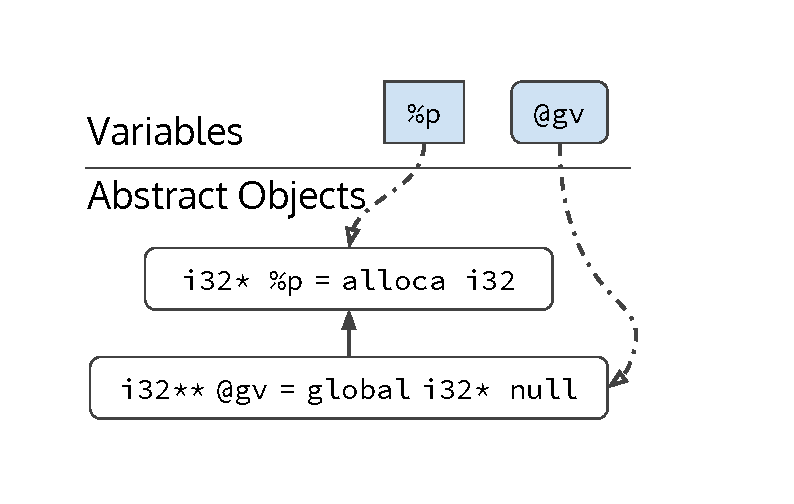
\includegraphics[trim={14mm 10mm 0 0},clip,width=1.5\linewidth]{figures/structsens/Partial-SSA.pdf}
    \subcaption{Points-to graph}
    \label{structsens/fig/partialssa:pt}
  \end{minipage}
  \caption{Partial SSA Example}
  \label{structsens/fig/partialssa}
\end{figure}


\section{Structure-Sensitive Approach}
\label{structsens/sect/approach}

Our analysis approach adds more detail to object abstractions, which
serve both as sources and as targets of points-to edges, allowing a
more detailed representation of the heap. Although our approach is
applicable to C/C++ analysis in general, it is best to see it in
conjunction with the LLVM bitcode intermediate language. Just as LLVM
bitcode is a strongly-typed intermediate language, we assign types and
offsets to every abstract object value and its points-to
relationships. The challenge is that, unlike in the LLVM bitcode type
system, such information is not readily available by local inspection
of the code---it needs to be propagated by the analysis reasoning
itself.

We next discuss the various abstractions of our analysis, in
representing its input and output relations. Then, we express the main
aspects of our analysis as a set of inference rules.

\subsection{Abstractions}
\label{structsens/sect/abstractions}

Figure~\ref{structsens/fig/domains} presents the input and output
domains of our analysis. We represent functions as a subset of global
entities. Thus, $G$ contains all symbols referencing global
entities---everything starting with symbol ``\code{@}'' in LLVM
bitcode. Set $V$ holds temporaries only (i.e., virtual registers), and
not global variables. We represent the union of these two sets with
$P$, which stands for \emph{pointer variables} (i.e., any entity whose
value may hold some memory address). Our analysis only introduces the
set of abstract objects $O$, that correspond to memory locations.

\begin{figure}[ht]
  \centering
  \begin{tabular}{l@{\quad}l}
    \toprule
    $T$ & set of program types \\
    $L$ & set of instruction labels \\
    $C$ & program (integer) constants \\
    $V$ & set of virtual registers \\
    $G$ & set of global variables \\
    $F \subseteq G$ & program functions \\
    $P = V \cup G$ & pointer variables \\
    \midrule
    $O$ & set of abstract objects \\
    \bottomrule
  \end{tabular}
  \caption{Analysis Domains}
  \label{structsens/fig/domains}
\end{figure}

The LLVM IR defines an extensive instruction set. However, only a
small subset is relevant for the purposes of pointer
analysis. Figure~\ref{structsens/fig/llvm} presents a simplified
version of these relevant instructions. The first two instructions are
used to allocate memory on the stack and on the heap, respectively. As
previously discussed, \instr{alloca} instructions are used for
address-taken variables. They accept an extra type argument (absent in
\instr{malloc} instructions), which specifies the exact type of the
allocation (virtual registers are strongly typed), and the allocation
size is a constant. Next, we have \instr{cast} instructions, used
solely to satisfy LLVM's type checker since they do not change any
memory contents, and \instr{phi} instructions that choose a value
depending on the instruction's predecessor. Apart from the standard
\instr{load}/\instr{store} instructions, we have two more instructions
that, given a memory address operand, return a new address by adding a
relative offset that corresponds to either a field or an array
element. (Only \instr{load} instructions dereference memory, however.)
Finally,
%% Not clear to me why store can take a constant address but load cannot.
%% If constants can be handled via intermediate registers in one case,
%% they also can in the other.
we have call and return instructions. Call instructions may also
accept a variable (function pointer), as their first argument.

\begin{figure}[t]
  \centering
  \begin{tabular}{l@{\quad}l@{\qquad}l}
    \toprule
    \emph{LLVM Instruction}
    & \emph{Operand Types}
    & \emph{Description} \\
    \midrule
    $\allocainstr{p}{T}{nbytes}$
    & $V \!\times\! T \!\times\! C$
    & Stack Allocations
    \\
    $\mallocinstr{p}{nbytes}$
    & $V \!\times\! (V \cup C)$
    & Heap Allocations
    \\
    $\castinstr{p}{T}{q}$
    & $V \!\times\! T \!\times\! (P \cup C)$
    & (No-op) Casts
    \\
    $\phiinstr{p}{l_1 : a_1}{l_2 : a_2}$
    & $V \!\times\! (L \mapsto (P \cup C))^2$
    & SSA Phi Node
    \\
    $\loadinstr{p}{q}$
    & $V \!\times\! P$
    & Load from Address
    \\
    $\storeinstr{p}{q}$
    & $P \!\times\! (P \cup C)$
    & Store to Address
    \\
    $\fieldaccess{p}{q}{f}$
    & $V \!\times\! P \!\times\! C$
    & Address-of-field
    \\
    $\arrayaccess{p}{q}{idx}$
    & $V \!\times\! P \!\times\! (V \cup C)$
    & Address-of-array-index
    \\
    $\callinstr{p}{a_0}[a_1][a_2,\ldots,a_n]$
    & $V \!\times\! (F \cup V) \!\times\! (P \cup C)^n$
    & Function Call
    \\
    $\returninstr{p}$
    & $P \cup C$
    & Function Return
    \\
    \bottomrule
  \end{tabular}
  \caption[LLVM IR Instruction Set]{%
    LLVM IR Instruction Set. We also prepend a label $l \in L$ to each
    instruction (that we omit in this figure). Each such label can be
    used to uniquely identify its instruction. %
  }
  \label{structsens/fig/llvm}
\end{figure}


\paragraph{Abstract Objects.}
Our analysis defines several different kinds of abstract objects that
express the exact nature of the allocation. Any abstract object must
fall into one of the following categories:

\begin{minipage}{\linewidth}
  \renewcommand{\arraystretch}{1.5}
  \begin{tabular}{@{--\ }l@{\quad}p{0.87\textwidth}}
    $\alloc{o_i}$
    & A stack or heap allocation for instruction (allocation site) $i \in L$.
    \\[3pt]
    $\alloc{o_{i,\tp{T}}}$
    & A (heap) allocation for instruction $i \in L$, specialized for type
      $\tp{T} \in T$.
    \\[3pt]
    % $\alloc{o_{v,i}}$
    % & A stack allocation for instruction (allocation site) $i \in L$,
    % assigned to virtual register $v \in V$.
    % \\[3pt]
    $\alloc{o_{g}}$
    & A global allocation for global variable or function $g \in G$.
    \\[3pt]
    % $\alloc{o_{f}}$
    % & A global allocation for function $f \in F$.
    % \\[3pt]
    $\alloc{o.fld}$
    & A field subobject that corresponds to field ``$fld\,$'' of base object
      $\alloc{o} \in O$.
    \\[3pt]
    $\alloc{o[c]}$
    & An array subobject that corresponds to the element at constant
      index $c \in C$ of base object $\alloc{o} \in O$.
    \\[1pt]
    $\alloc{o[*]}$
    & An array subobject that corresponds to any elements at unknown
      indices of base object $\alloc{o} \in O$.
    \\
  \end{tabular}
\end{minipage}

\noindent
When not using any special notation, we shall refer to a generic
abstract object that could be of any of the above forms. This also
applies to the base object of the last three categories (which, thus,
serve as recursive definitions), allowing us to define arbitrarily
complex subobjects such as \(\alloc{o.f[4].g[*]}\).

By representing field and array subobjects as separate abstract
objects themselves, the handling of instructions that return addresses
anywhere but at the beginning of some allocation becomes
straightforward. As we shall see at
Section~\ref{structsens/sect/rules}, all our analysis has to do is
return the relevant abstract object that represents the given
subobject of its base allocation. This abstract subobject will have
its own distinct points-to set, which will be tracked separately from
that of its base allocation or any of the rest of its fields. Thus, it
will allow the analysis to retain a certain degree of precision that
would be otherwise impossible.
% for a field-insensitive approach.

\vspace{0.5em}
\noindent
Our analysis computes four main
relations:
\begin{description}
\item[Variable points-to edges.] Edge $\vpt{p}{o} \in P \times O$
  records that pointer variable (either virtual register or global
  variable) $\var{p}$ may point to abstract object $\alloc{o}$. Note
  that virtual registers that correspond to source variables will
  always point to a single object: the corresponding stack
  allocation. Temporaries introduced by LLVM bitcode, though, may
  point to many abstract objects.
\item[Dereference edges.] Edge $\derefpt{po}{o} \in O \times O$
  records that abstract object $\alloc{po}$ may point to abstract
  object $\alloc{o}$. Any object that has a non-empty points-to set
  (i.e., the object has outgoing dereference edges) may represent a
  pointer. Dereference edges can only be established by \instr{store}
  instructions.
\item[Abstract object types.] The partial function
  $\typefunc: O \nrightarrow T$ records the type of an abstract
  object. An abstract object can be associated with one type at most,
  or none at all. Since our analysis uses types to filter redundant
  derivations, the more types it establishes for abstract objects, the
  more points-to edges it will compute.
  %
  Figure~\ref{structsens/fig/typeinf} establishes some basic type
  relations between the subobjects created by the analysis.
\item[Call-graph edges.] Edge $i \xrightarrow{calls} f \in L \times F$
  records that invocation site $i$ may call function $f$. This also
  accounts for indirect calls that use function pointers.
\end{description}

\begin{figure}[t]
  \begin{math}
    \inferrule* [left=Struct Type\;]
    {\alloctype{o} = \tp{S}
      \\ \gtype{\tp{S}.f} = \tp{F}}
    {\alloctype{o.f} = \tp{F}}
  \end{math}
  \;
  \begin{math}
    \inferrule* [left=Array Type\;]
    {\alloctype{o} = [\tp{T}]
      \\ c \in C}
    {\alloctype{o[*]} = \tp{T}
      \\ \alloctype{o[c]} = \tp{T}}
  \end{math}
  \caption{Basic Type Inferences for Abstract Objects.}
  \label{structsens/fig/typeinf}
\end{figure}


\subsection{Techniques - Rules}
\label{structsens/sect/rules}

Figure~\ref{structsens/fig/rules} presents the main aspects of the
analysis as a set of inference rules. The first two rules handle stack
and heap allocation instructions. All they do is create a new abstract
object representing the given allocation site, and assign it to the
target variable. In the case of stack allocation, we also record the
type of the object, since it is available at the allocation site. The
next pair of rules handle global allocations for global variables and
functions, respectively, in a similar way. In contrast to the previous
rules, we create abstract objects for all global entities, regardless
of any instructions (since their allocation in LLVM bitcode is
implicit), and record their types.

\begin{figure}[h!t]
  \begin{math}
    \inferrule* [left=Stack\;]
    {\allocainstr[i]{p}{T}{nbytes}}
    {\vpt{p}{o_{i}}
      \\ \alloctype{o_{i}} = \tp{T}}
  \end{math}
  \qquad
  \begin{math}
    \inferrule* [left=Heap\;]
    {\mallocinstr[i]{p}{nbytes}}
    {\vpt{p}{o_{i}}}
  \end{math}
  \\

  \begin{math}
    \inferrule* [left=Global\;]
    {\constant{f} \in F}
    {\cpt{f}{o_f}
      \\ \alloctype{o_f} = \gtype{f}}
    \qquad
    \inferrule*
    {\var{g} \in (G \setminus F)
      \\ \vartype{g} = \tp{T\,*}}
    {\vpt{g}{o_g}
      \\ \alloctype{o_g} = \tp{T}}
  \end{math}
  \\
  % \begin{math}
  %   \inferrule* [left=Field\;]
  %   {\alloctype{o} = \tp{S}
  %   \\ \exists \, \code{\tp{S}.fld}}
  %   {\exists \, \alloc{o.fld}
  %   \\ \alloctype{o.fld} = \codetype{\tp{S}.fld}}
  % \end{math}
  % \\

  % \begin{math}
  %   \inferrule* [left=Array\;]
  %   {\alloctype{o} = \tp{[T$\times$N]}}
  %   {\exists \, \alloc{o[*]}
  %   \\ \alloctype{o[*]} = \tp{T}}
  %   \quad
  %   \inferrule*
  %   {\alloctype{o} = \tp{[T$\times$N]}
  %   \\ \arrayaccess[i]{p}{q}{c}
  %   \\ \vartype{q} = \alloctype{o}}
  %   {\exists \, \alloc{o[c]}
  %   \\ \alloctype{o[c]} = \tp{T}}
  % \end{math}
  % \\
  \begin{math}
    \inferrule* [left=Cast\;]
    {\castinstr[i]{p}{T}{q}
      \\ \vpt{q}{o}}
    {\vpt{p}{o}}
  \end{math}
  \qquad
  \begin{math}
    \inferrule* [left=Phi\;]
    {\phiinstr[i]{p}{l_1 : a_1}{l_2 : a_2}}
    {\forall j:\ \opt{a_j}{o} \;\Rightarrow\; \opt{p}{o}}
  \end{math}
  \\

  \begin{math}
    \inferrule* [left=Load\;]
    {\loadinstr[i]{p}{q}
      \\ \vpt{q}{po}
      \\ \derefpt{po}{o}}
    {\vpt{p}{o}}
  \end{math}
  \quad
  \begin{math}
    \inferrule* [left=Store\;]
    {\storeinstr[i]{p}{q}
      \\ \vpt{p}{po}
      \\ \vpt{q}{o}}
    {\derefpt{po}{o}}
  \end{math}
  \\

  \begin{math}
    \inferrule* [left=Field\;]
    {\fieldaccess[i]{p}{q}{f}
      \\ \vpt{q}{o}
      \\ \alloctype{o} = \tp{S}
      % TODO consider adding \\ f \in \fields{S}
      \\ \vartype{q} = \tp{S\,*}}
    {\vpt{p}{o.f}}
  \end{math}
  \\

  \begin{math}
    \inferrule* [left=Array -- Const\;]
    {\arrayaccess[i]{p}{q}{c}
      \\ \vpt{q}{o}
      \\ \alloctype{o} = [\tp{T}]
      \\ \vartype{q} = [\tp{T}]\,\code{*}}
    {\vpt{p}{o[c]}}
  \end{math}
  \\

  \begin{math}
    \inferrule* [left=Array -- Var\quad \;]
    {\arrayaccess[i]{p}{q}{\var{j}}
      \\ \vpt{q}{o}
      \\ \alloctype{o} = [\tp{T}]
      \\ \vartype{q} = [\tp{T}]\,\code{*}}
    {\vpt{p}{o[*]}}
  \end{math}
  \\
  
  \begin{math}
    \inferrule* [left=Call\;]
    {\callinstr[i]{p}{a_0}[a_1][a_2,\ldots,a_n]
      \\ \opt{a_0}{o_f}
      \\ f \in F }
    {i \xrightarrow{calls} f(\op{p_1},\, \op{p_2},\, \ldots,\,
      \op{p_n})
      \\ \forall j:\ \opt{a_j}{o} \;\Rightarrow\; \opt{p_j}{o}}
  \end{math}
  \\

  \begin{math}
    \inferrule* [left=Ret\;]
    {\callinstr[i]{p}{a_0}
      \\ i \xrightarrow{calls} f(\ldots)
      \\ \returninstr[j]{q}
      \\ j \in \body{f}
      \\ \vpt{q}{o}}
    {\vpt{p}{o}}
  \end{math}
  \\

  \begin{math}
    \inferrule* [left=Heap-bp\;]
    {\mallocinstr[i]{p}{nbytes}
      \\ \castinstr[j]{w}{T\,*}{q}
      \\ \vpt{q}{o_{i}}}
    {\vpt{p}{o_{i,\tp{T}}}
      \\ \alloctype{o_{i,\tp{T}}} = \tp{T}}
  \end{math}
  \caption{Inference Rules}
  \label{structsens/fig/rules}
\end{figure}


For cast instructions, we copy any object that flows in the points-to
set of the source variable to the points-to set of the target
variable. Phi instructions are treated similarly, but we have to
consider both of the instruction's operands, regardless of their
corresponding labels, since our result must be an
over-approximation.

% Stores
Store instructions are the only way in which the analysis establishes
dereference edges. For a store instruction, $\storeinstr{p}{q}$, we have
to perform the following:% steps:

\begin{enumerate}
\item First, find the corresponding abstract objects that the two
  instruction operands point to, by following their outgoing variable
  points-to edges. Namely:
  \begin{inparaenum}[(i)]
  \item the memory allocation of the value to be stored (abstract
    object $\alloc{o}$), and
  \item the memory allocation that $\alloc{o}$ is going to be stored
    into (abstract object $\alloc{po}$).
  \end{inparaenum}
\item Then, establish a dereference edge between any two such abstract
  objects returned, expressing that object $\alloc{po}$ may point to
  object $\alloc{o}$.
\end{enumerate}
The first step simply bypasses the indirection introduced by LLVM
bitcode, where operands are represented as virtual registers that
point to memory locations.
% Loads
Load instructions perform the opposite operation, and thus are treated
symmetrically. For instruction $\loadinstr{p}{q}$, we first
\begin{inparaenum}[(i)]
\item find the corresponding abstract object that the address operand
  may point to (abstract object $\alloc{po}$),
\item then follow any outgoing dereference edge of object $\alloc{po}$
  to get any memory location $\alloc{po}$ may point to (object
  $\alloc{o}$), and finally
\item establish a new variable points-to edge for target variable
  $\var{p}$, recording that $\var{p}$ may now also point to object
  $\alloc{o}$.
\end{inparaenum}

The next three rules (\textsc{Field, Array--Const, Array--Var}) model field sensitivity. The rule
handling field accesses, such as $\fieldaccess{p}{q}{f}$, finds any
object $\alloc{o}$ that base variable $\var{q}$ may point to, and
returns $\alloc{o}\,$'s relevant field subobject
$\alloc{o.f}$. However, a key element is that $\alloc{o}$
is only considered as a base object if its type matches the declared
(struct) type of $\var{q}$ (recall that LLVM bitcode is strongly
typed). This precludes any untyped heap allocations as possible base
objects. Otherwise, the analysis would end up creating untyped field
subobjects too, further fueling imprecision. Thus, we are able to
maintain an important invariant of our structure-sensitive analysis:
\emph{only create field (or array) subobjects whose types we are able
  to determine}. Effectively, LLVM bitcode  imposes
\emph{strong typing on variables}, while our analysis extends the treatment
to \emph{abstract objects}.

Array element accesses are treated similarly and they, too, maintain
this invariant. However, we distinguish array accesses using a
constant index from those using a variable (i.e., unknown)
index. In the former case, we return the array subobject
$\alloc{o[c]}$, which represents the subobject at index
$c$. In the latter case, we return $\alloc{o[*]}$, which represents
the \emph{unknown} index. Essentially, this treatment allows our
analysis to track independently the points-to sets of array indices that are
statically known to be different, yielding a form of
\emph{array-sensitivity}.

Call and return instructions as modeled as assignments:
\begin{inparaenum}[(i)]
\item from any actual argument $a_j$ to its respective formal
  parameter $f_j$, and
\item from any returned value $\var{q}$ to the target variable of the
  call instruction $\var{p}$.
\end{inparaenum}
Like cast instructions, they simply copy the points-to sets from the
assignment's source to its target. However, the rule that handles call
instructions also records call-graph edges. When the function operand
$a_0$ may point to abstract object $o_f$, representing function $f$,
we record an edge from the given call site to function $f$. This
handles both direct and indirect calls (i.e., via function pointers).
% REVIEW: not entirely accurate; implementation uses filters on this
% case
% Note that no type checking needs to be performed by the analysis at
% this point. The type correctness of the call is ensured by the LLVM
% bitcode type system.

\paragraph{How to produce type information for unknown objects.}
%Allocation-site+Type Abstraction.}
Our analysis only allows taking the address of fields of objects 
whose type is known. This prevents loading and storing from/to fields
of objects without types. Such objects can only be used as identity
markers. Yet C and C++ allow the creation of untyped objects. Their handling
is a key element of the analysis.

The \textsc{Heap-bp} rule implements the \emph{use-based
back-propagation} technique~\cite{ecoop/LiTSX14,aplas/LivshitsWL05,aplas/SmaragdakisBKB15}, which creates multiple abstract
objects per (untyped) allocation site. The rule states that when an (untyped)
heap object $\alloc{o_i}$ (allocated at instruction $i$)
flows to some cast instruction $j$, where it is cast to type \tp{T}, we
augment the points-to set of $i$'s target variable $\var{p}$ with a
new abstract object $\alloc{o_{i,\tp{T}}}$, specialized for the given
type. The insight behind this rule is that, even when the program
performs an allocation via a type-agnostic routine like
\code{malloc()}, the allocation will be later cast to its intended
type before being used. By using this technique, the original untyped
allocation will be prevented from creating any untyped subobjects, but
as soon as the possible type of the allocation is discovered, the new
abstract typed object will succeed where the untyped one has failed.
Note that instructions $i$ and $j$ 
%are in no way related. They
could occur in distant parts of the program, as long as the analysis
can establish that the object allocated at instruction $i$ flows to
$j$.

This treatment successfully deals with generic
allocation wrappers or factory methods. In this case, the wrapped
allocation will flow to multiple cast instructions, and thus create
multiple typed variations of the original object. However, in each
case, only the object with the correct matching type will be used as a
base for any subsequent address-of-field instructions.
The rest of the objects will be filtered, since they are
indeed irrelevant.


\subsection{Partial Order of Abstract Objects}

As the observant reader may have noticed, the rules of
Figure~\ref{structsens/fig/rules} about accesses or array elements are
not sound. Consider the example of
Figure~\ref{structsens/fig/array}. Variable $\var{p}$ points to a heap
allocation. Three different store instructions take place:
\begin{inparaenum}[(i)]
\item one that stores $\code{\&i}$ to index 1,
\item one that stores $\code{\&j}$ to index 3, and
\item one that stores $\code{\&k}$ to some variable index.
\end{inparaenum}
When loading from index 1, the analysis has to return both
$\code{\&i}$ and $\code{\&k}$ (since the value of variable $\var{idx}$
may be equal to 1), but not $\code{\&j}$, which is stored to a
different index. Conversely, when loading from a variable index, the
analysis has to return all three addresses, since the index could be
equal to any constant.

\begin{figure}[ht]
\begin{cppcode}
int i, j, k, idx;
...
int **p = malloc(...);
p[1] = &i;
p[3] = &j;
p[idx] = &k;
int *x = p[1];  // yields $\{ i, k \}$
int *y = p[2];  // yields $\{ k \}$
int *z = p[j];  // yields $\{ i, j, k \}$
\end{cppcode}
  \caption{Accessing array elements.}
  \label{structsens/fig/array}
\end{figure}

Using our array-sensitive approach, we ensure that indices 1, 3, and
``$*$'' (unknown) are associated with separate points-to sets that are
not merged. To handle loads correctly, though, we have to be able to
reason about implicit associations of abstract objects, due to
possible index aliases. Thus, we say that object
$\alloc{o[*]}$ ``generalizes'' object $\alloc{o[c]}$ (for the same
base object $\alloc{o}$), since loading from $\alloc{o[*]}$ must
always return a superset of the objects returned by loading from
$\alloc{o[c]}$, for any constant $c$. This concept extends even to
deeply nested subobjects. For instance, an object 
$\alloc{o.f_1[*][2].f_2[*]}$ generalizes object
$\alloc{o.f_1[4][2].f_2[*]}$.

We can think of this binary relation between abstract objects as a
partial order over domain $O$ and define it appropriately.

\begin{defn}{\emph{Abstract Object Generalization Order.}}
  An abstract object $\alloc{y} \in O$ \emph{generalizes} an abstract
  object $\alloc{x}$, denoted $\alloc{x} \sqsubseteq \alloc{y}$, if
  and only if:

\begin{gather*}
  \alloc{x} = \alloc{y}
  \\
  \lor
  \\
  (\, \alloc{x} = \alloc{p[*]}\ \lor\ \alloc{x} = \alloc{p[c]} \,)\
  \land\ \alloc{y} = \alloc{q[*]}\
  \land\ \alloc{p} \sqsubseteq \alloc{q}
  \\
  \lor
  \\
  (\alloc{x} = \alloc{p.f}\
  \land\ \alloc{y} = \alloc{q.f}\
  \land\ \alloc{p} \sqsubseteq \alloc{q})
  \\
  \lor
  \\
  (\alloc{x} = \alloc{p[c]}\
  \land\ \alloc{y} = \alloc{q[c]}\
  \land\ \alloc{p} \sqsubseteq \alloc{q})
\end{gather*}
\end{defn}

\noindent
Intuitively, $\alloc{o_1} \sqsubseteq \alloc{o_2}$ holds when
$\alloc{o_1}$ can be turned to $\alloc{o_2}$ by substituting any of
its constant array indices with
``$*$''. Figure~\ref{structsens/fig/poset} gives an example of such
ordering. The direction of the edges is from the less to the more
general object.

\begin{figure}[ht]
  \centering
  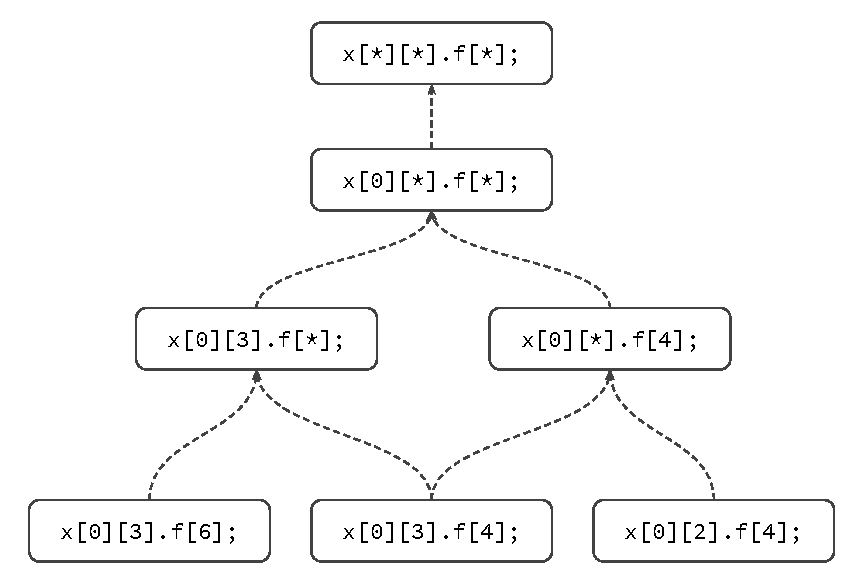
\includegraphics[clip,width=0.80\linewidth]{figures/structsens/Partial-Order.pdf}
  \caption[Abstract Object Ordering]{%
    Abstract Object Ordering -- Example: Nodes are abstract
    objects. An edge $(\, \alloc{s},\alloc{t} \,)$ denotes that object
    $\alloc{s}\:$ is generalized by object $\alloc{t}\:$ (i.e.,
    $\, \alloc{s} \sqsubseteq \alloc{t}\, $).}
  \label{structsens/fig/poset}
\end{figure}

Given this partial order, it suffices to add the two rules of
Figure~\ref{structsens/fig/rules:star} to account for possible index
aliases. The first rule states that the points-to set of a (less
general) object, such as $\alloc{o[c]}$, is a superset of the
points-to set of any object that generalizes it, such as
$\alloc{o[*]}$. The second rule modifies the treatment of load
instructions, so that they may return anything in the points-to set of
not just the object we load from (such as $\alloc{o}[*]$), but also of
objects that it generalizes (such as $\alloc{o[c]}$). In this way, the
general and specific points-to sets are kept distinct, while their
subset relationship is maintained.

\begin{figure}[ht]
  % \begin{math}
  %   \inferrule*
  %   {\alloc{o} \in O}
  %   {\alloc{o} \le \alloc{o}}
  % \end{math}
  % \quad
  % \begin{math}
  %   \inferrule*
  %   {\alloc{o_1} \le \alloc{o_2}
  %     \\ \alloc{o_1[c]}, \alloc{o_2[*]} \in O}
  %   {\alloc{o_1[c]} \le \alloc{o_2[*]}}
  % \end{math}
  % \\
  % \begin{math}
  %   \inferrule*
  %   {\alloc{o_1} \le \alloc{o_2}
  %     \\ \alloc{o_1.f}, \alloc{o_2.f} \in O}
  %   {\alloc{o_1.f} \le \alloc{o_2.f}}
  % \end{math}
  % ~
  % \begin{math}
  %   \inferrule*
  %   {\alloc{o_1} \le \alloc{o_2}
  %     \\ \alloc{o_1[c]}, \alloc{o_2[c]} \in O}
  %   {\alloc{o_1[c]} \le \alloc{o_2[c]}}
  % \end{math}
  % ~
  % \begin{math}
  %   \inferrule*
  %   {\alloc{o_1} \le \alloc{o_2}
  %     \\ \alloc{o_1[*]}, \alloc{o_2[*]} \in O}
  %   {\alloc{o_1[*]} \le \alloc{o_2[*]}}
  % \end{math}
  % \\
  \begin{math}
    \inferrule* [left=Match\;]
    {\alloc{o_1} \sqsubseteq \alloc{o_2}
      \\ \derefpt{o_2}{o}}
    {\derefpt{o_1}{o}}
  \end{math}
  \quad
  \begin{math}
    \inferrule* [left=Load II\;]
    {\loadinstr[i]{p}{q}
      \\ \vpt{q}{o_2}
      \\ \alloc{o_1} \sqsubseteq \alloc{o_2}
      \\ \derefpt{o_1}{o}}
    {\vpt{p}{o}}
  \end{math}
  \\
  \caption{Associating array subobjects via their partial order.}
  \label{structsens/fig/rules:star}
\end{figure}


\subsection{Soundness}

As stated by Avots et al. \cite{icse/AvotsDLL05}: ``\textit{A C
  pointer alias analysis cannot be strictly sound, or else it would
  conclude that most locations in memory may point to any memory
  location.}''
%
As in the PCP points-to analysis \cite{icse/AvotsDLL05}, our approach
tries to maintain precision at all times, even if this means that the
analysis is not sound in some cases.
%
Instead of trying to be as conservative as possible, we choose to opt
for precision and increase soundness by selectively supporting
well-established code patterns or idioms (such as using
\code{malloc()} to allocate many objects of different types).
%

The soundness assumptions of our analysis are that:
\begin{inparaenum}[(i)]
\item objects are allocated in separate memory spaces
  \cite{icse/AvotsDLL05}, and 
\item every (concrete) object has a single type throughout its
  lifetime.
\end{inparaenum}
%
Hence, our analysis would be unsound when a union type is used to
modify the same concrete object using two different types, since this
violates the second assumption. However, our analysis would be a good fit for
programs that use \emph{discriminated unions} (e.g., unions that
depend on a separate \emph{tag} field to determine the exact type of
the object), since it would create a different abstract object for
every type of the union, so that each such abstract object would
represent the subset of concrete objects with the same tag value.

In general, the single-type-per-lifetime assumption is reasonable for
most objects, but would be prohibitive in some cases---especially so
when the code relies on low-level assumptions about the byte layout of
the objects. For instance, our base approach would not be able to
meaningfully analyze code that uses a custom memory
allocator. Instead, the analysis would need to be extended so that it
models calls to the allocator by creating new abstract objects.

Finally, the analysis must be able to discover all associated types
for any given object, to retain its soundness. For simplicity, we
have only considered cast instructions as places where the
analysis discovers new types, but it is easy to supply additional type
hints by considering more candidates. For instance, an
exception object of unknown type may be allocated and then thrown, by
calling the \code{cxa::throw()} function in the C++ exception handling
ABI, without any intervening cast. However, we can use the
accompanying \emph{typeinfo} object (always supplied as the second
argument to \code{cxa::throw()}) to recover its true type and hence
create a typed abstract exception object. To the best of our
knowledge, such special treatment is needed only in rare cases, and
the analysis can be easily extended to handle them.


\section{Analyzing C++}
\label{structsens/sect/cxx}

LLVM bitcode is a representation well-suited for C. However, for OO
languages such as C++, high-level features are
translated to low-level constructs.  A classic example is dynamic
dispatch, through virtual methods. Virtual-tables are represented as
constant arrays of function pointers, and virtual calls are, in turn,
translated to a series of indirect access instructions.

\begin{figure}[ht]
  \begin{minipage}[b]{.5\linewidth}
%define void @func() {
% %b=alloca %class.B, // B b;
% ...
%
%}

\begin{bitcode}
%class.B = type { i32 (...)**, ...}

;; translation of bp->foo(), for
;; B *bp;
%1 = bitcast %bp to i32 (%class.B*)***
%2 = load i32 (%class.B*)** %1
%3 = getelementptr i32 (%class.B*)** %2, 1
%4 = load i32 (%class.B*)* %3
call i32 %4 (%class.B* %bp)
\end{bitcode}
    \subcaption{C++ virtual call compiled to LLVM bitcode}
    \label{structsens/fig/vcall:bitcode}
  \end{minipage}
  \begin{minipage}[b]{.5\linewidth}
    \centering
    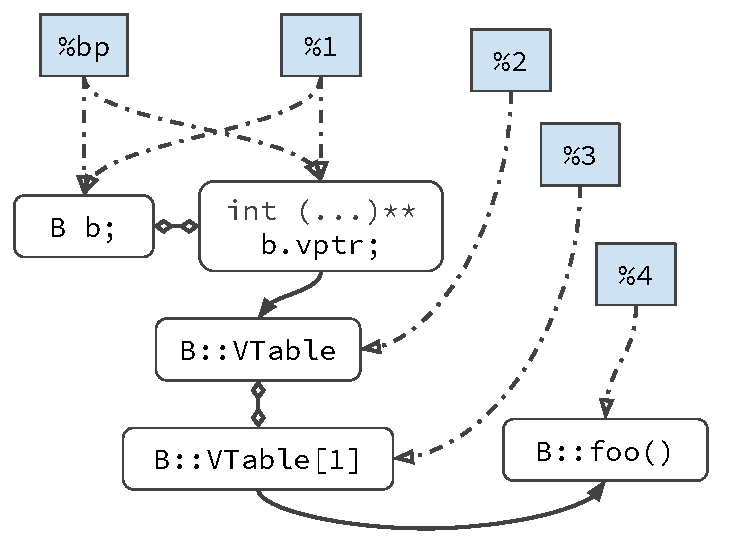
\includegraphics[trim={0 0 0 0},clip,width=1\linewidth]{figures/structsens/Virtual-Call.pdf}
    \subcaption{Points-to graph}
    \label{structsens/fig/vcall:ptgraph}
  \end{minipage}
  \caption{C++ Virtual Call Example}
  \label{structsens/fig/vcall}
\end{figure}

Figure~\ref{structsens/fig/vcall:bitcode} presents (a simplified
version of) the LLVM bitcode for such a translation. A virtual call
has to
\begin{inparaenum}[(i)]
\item load the v-pointer of the class instance (at offset 0),
\item index into the returned v-table (at the corresponding offset of
  the function being called),
\item then load the returned function pointer to get the exact address
  of the function, and
\item finally call the function.
\end{inparaenum}
By employing the techniques we have described so far, our
structure-sensitive analysis is well-equipped to deal with such an
involved pattern, and precisely resolve the function to be called.

Figure~\ref{structsens/fig/vcall:ptgraph} shows what our analysis
computes (assuming $\var{\%bp}$ points to variable $\var{b}$). Only a
minor addition is required: anything that points to an object should
also point to its first field (at byte offset 0). Hence, both
$\var{\%bp}$ and $\var{\%1}$ (after the cast) will point both to
(stack-allocated) object $\alloc{b}$, and to its v-pointer field
subobject $\alloc{b.vptr}$. The first load instruction will return the
v-table. Indexing into the v-table will return the corresponding array
element subobject, which will maintain its own independent (singleton)
points-to set, due to array-sensitivity. Finally, the second load
instruction will return the exact function that the v-table points to,
at the given offset.


\section{Enhancements}
\label{structsens/sect/addons}

Section~\ref{structsens/sect/approach} presented only the essential
parts of a structure-sensitive points-to analysis, but there can be
many enhancements worth discussing at this point. In this section, we
will list a few of the most valuable ones for a practical
implementation.

\subsection{Pointer Arithmetic}

In C/C++, given a pointer ``\mintinline{c++}{P *ptr}'', expressions
such as
\begin{inparaenum}[(i)]
\item ``\mintinline{c++}{(*ptr).fld}'',
\item ``\mintinline{c++}{ptr->fld}'', and
\item ``\mintinline{c++}{ptr[0].fld}''
\end{inparaenum}
are equivalent (and will be translated to the same LLVM bitcode
instruction). Hence, a pointer analysis must be able to reason about
such code patterns and map them to the same abstract (sub)object. In
LLVM IR, all such field accesses would be canonicalized to the third
form. In fact, all pointers in LLVM bitcode are treated as pointers to
arrays of objects (even when they point to a single
one).\footnote{This is exactly the reason for the first (frequently
  zero) index of the often misunderstood \code{getelementptr} LLVM
  bitcode instruction (see
  \url{http://llvm.org/docs/GetElementPtr.html}).}  Regarding the
possible choices of analysis inputs (discussed in
Chapter~\ref{chapter:intro}), such translations are certainly a point
in favor of choosing an intermediate representation such as LLVM
bitcode, so that the analysis need not concern itself with superfluous
syntactic constructs.

However, we have not so far delved into the various pointer arithmetic
idioms that are supported by C/C++ and that we would like for our
structure-sensitive analysis to support as well. A pointer in C is a
memory address, which is a numeric value. One can perform arithmetic
operations on a pointer just as with other numeric values. For
instance, the expression ``\mintinline{c++}{ptr+3}'' is equivalent to
``\mintinline{c++}{&ptr[3]}'' (which corresponds to the aforementioned
3rd form, as per LLVM's canonicalization).  Again LLVM's translation
can be very helpful in narrowing the complexity of the input
language. To see how our analysis can be extended to support pointer
arithmetic, we first have to briefly present LLVM's GEP instruction,
since this is what all types of element accesses (and pointer
arithmetic operations) are normally translated to.

\paragraph{The GEP Instruction.} The actual LLVM bitcode instruction
that is responsible for all types of element accesses is
\instr{getelementptr} (GEP). The GEP instruction accepts a base
pointer argument and one or more index arguments. It can be used to
retrieve any inner element of an arbitrarily nested structure. Its
general form is:

\[
  \mintinline{llvm}{
    %ptr = getelementptr %base, %idx1, %idx2, %idx3,
  }
  \ldots
\]

Assuming that \code{\%base} may point to an array of objects (in the
general case), the first index selects an element of this
array. (Expressions such as ``\mintinline{c++}{ptr->fld}''---being
equivalent to ``\mintinline{c++}{ptr[0].fld}''---implicitly refer to
the first element and thus produce a zero first index.)
%
Any index after the first corresponds to a field or array element
access.
% A variable can only be used in place of \code{\%idx1} (to
% index into the base pointer) or in any subsequent array indices (as
% opposed to field indices that always require a constant index).
Even
though the generic form of GEP may contain multiple indices to be able
to return the address of deeply nested elements, in practice, such
complex GEP instructions are split into multiple chained GEPs with at
most 2 indices.
%
Each one will descend in a single field or array index, roughly
corresponding to the \emph{address-of-field} and
\emph{address-of-array-index} instructions that we have previously
shown. Returning the address corresponding to a complex access path
such as ``\mintinline{c++}{ptr->f[4].g[k]}'' will require as many GEPs
as the depth of the access path: two field and two array accesses,
four in total.
%
Note that GEP instructions do not perform any memory dereference (as
the \instr{load} instruction does), but only compute a relative
offset.

So far we have not examined GEP instructions whose first index is
non-zero (thus retrieving the address of an element other than the
first, given a base pointer array). Fortunately, we can further
decompose such instructions to a GEP instruction with a single
non-zero index and a second GEP instruction of 2 indices, whose first
index is always zero.

\begin{figure}[h!t]
  \centering
  \begin{minipage}[b]{.4\linewidth}
    \centering
    \begin{bitcode}
      %ptr = getelementptr %b, 7, %v1, 8
    \end{bitcode}
    \subcaption{Complex GEP instruction}\label{structsens/fig/gep1}
  \end{minipage}%
  \qquad
  \begin{minipage}[b]{.4\linewidth}
    \centering
    \begin{bitcode}
      %t1 = getelementptr %b, 7
      %t2 = getelementptr %t1, 0, %v1
      %ptr = getelementptr %t2, 0, 8
    \end{bitcode}
    \subcaption{Decomposed GEP instruction}
    \label{structsens/fig/gep2}\par\vfill
  \end{minipage}
  \caption{Decomposition of GEP instructions}
  \label{structsens/fig/gep}
\end{figure}

Figure~\ref{structsens/fig/gep} demonstrates such a decomposition that
breaks a complex GEP instruction into multiple simpler ones. The last
two instructions of the decomposed version of
Figure~\ref{structsens/fig/gep2} correspond to our familiar notions of
\emph{address-of-array-index} and \emph{address-of-field}
instructions. Thus, we can dispense with GEP's overloaded behavior and
keep our inference rules almost intact. However, we have to augment
the analysis to support a single-index GEP, just like the first
instruction of Figure~\ref{structsens/fig/gep2}. Essentially, such
instructions perform a pointer increment operation and are of special
interest, since they alone should suffice for most translations of
dynamically allocated arrays and pointer arithmetic operations that
we are interested in.

\begin{figure}[h!t]
  \begin{math}
    \inferrule* [left=Stack\;]
    {\allocainstr[i]{p}{T}{nbytes}}
    {\vpt{p}{o_{i}[0]}
      \\ \alloctype{o_{i}[0]} = \tp{T}}
  \end{math}
  \qquad
  \begin{math}
    \inferrule* [left=Heap\;]
    {\mallocinstr[i]{p}{nbytes}}
    {\vpt{p}{o_{i}[0]}}
  \end{math}
  \\

  \begin{math}
    \inferrule* [left=Pointer -- Var I\quad \;]
    {\ptraccess[i]{p}{q}{\var{j}}
      \\ \gtype{q} = \tp{T\,*}
      \\ \vpt{q}{o[k]}
      \\ \alloctype{o[k]} = \tp{T}}
    {\vpt{p}{o[*]}}
  \end{math}
  \\

  \begin{math}
    \inferrule* [left=Pointer -- Var II\quad \;]
    {\ptraccess[i]{p}{q}{\var{j}}
      \\ \gtype{q} = \tp{T\,*}
      \\ \vpt{q}{o[*]}
      \\ \alloctype{o[*]} = \tp{T}}
    {\vpt{p}{o[*]}}
  \end{math}
  \\

  \begin{math}
    \inferrule* [left=Pointer -- Const I\;]
    {\ptraccess[i]{p}{q}{c}
      \\ \gtype{q} = \tp{T\,*}
      \\ \vpt{q}{o[*]}
      \\ \alloctype{o[*]} = \tp{T}}
    {\vpt{p}{o[*]}}
  \end{math}
  \\

  \begin{math}
    \inferrule* [left=Pointer -- Const II\;]
    {\ptraccess[i]{p}{q}{c}
      \\ \gtype{q} = \tp{T\,*}
      \\ \vpt{q}{o[k]}
      \\ \alloctype{o[k]} = \tp{T}
      \\\\  k + c \in \indices{T}}
    {\vpt{p}{o[k+c]}}
  \end{math}
  \\

  \begin{math}
    \inferrule* [left=Pointer -- Const III\;]
    {\ptraccess[i]{p}{q}{c}
      \\ \gtype{q} = \tp{T\,*}
      \\ \vpt{q}{o[k]}
      \\ \alloctype{o[k]} = \tp{T}
      \\\\  k + c \notin \indices{T}}
    {\vpt{p}{o[*]}}
  \end{math}
  \caption{Dealing with pointer arithmetic}
  \label{structsens/fig/ptrarithm}
\end{figure}

Figure~\ref{structsens/fig/ptrarithm} presents an extension of our
analysis to handle such pointer increment operations. The first two
rules replace the previous ones (for base allocations) by slightly
changing the objects we allocate to resemble the first
elements of potential array allocations. In cases where an instruction
allocates a single object, such zero offsets may be redundant but
facilitate the increment operations of the following rules. The next
two rules handle pointer increment operations that use a variable
index \(\var{j}\). In both cases, the result should disregard any
prior index of the object pointed by \var{q}, and replace it with the
``\(*\)'' index. The last three rules handle pointer increment
operations that add a constant \(c\). The first of them states that
adding a constant index to an already unknown index makes no
difference and simply propagates the same special object
(\(\alloc{o[*]}\)). In the last two rules, \(\var{q}\) points to an
object with a constant index instead (\(\alloc{o[k]}\)), whereupon the
analysis tries to compute a new constant index \(k+c\) and point to
the relevant object (\(\alloc{o[k+c]}\)). However, such general
treatment could potentially lead to the creation of infinite
objects. To avoid this, we only point to \(\alloc{o[k+c]}\) if the new
index \(k+c\) statically appears in the source code (and is associated
with type \(\tp{T}\)). Otherwise, the analysis falls back to using
\(\alloc{o[*]}\).

To identify what static indices are associated with each type we
define the function \emph{indices} as follows:
\begin{equation*}
  \begin{split}
    \indices{T} =
    \{ 0 \}
    & \cup
    \{ c :  \exists \; \ptraccess{p}{q}{c} \,\land\, \gtype{q} = \tp{T\,*}
    \}
    \\
    & \cup \{ c :  \exists \; \arrayaccess{p}{q}{c} \,\land\, \gtype{q} = [\tp{T}]
    \}
  \end{split}
\end{equation*}


\subsection{Abstract Object Aliases}

There are cases where two abstract objects, such as \(\alloc{o}\) and
\(\alloc{o[0]}\) may coincide (i.e., map to the same memory
address). This applies to both zero indices of arrays and the first
fields of structs. Ignoring such object aliases could lead to unsound
results, e.g., when dereferencing an object without taking the
points-to sets of its aliases into account.

To handle such cases, the analysis should treat aliased abstract
objects as an equivalence class.

\begin{defn}{\emph{Abstract Object Aliases.}}
  We define the \emph{alias} equivalence relation \(\sim\) on the set
  of abstract objects \(O\) as the transitive, symmetric, and
  reflexive closure of the binary relation \(\simless\), so that given
  two abstract objects \(\alloc{x},\, \alloc{y} \in O\),
  \(\alloc{x}\, \simless\; \alloc{y}\), if and only if:
  \begin{gather*}
    \alloc{y} = \alloc{x[0]}
    \\
    \lor
    \\
    \alloc{y} = \alloc{x.f} \land \offsetof(f) = 0
  \end{gather*}
  where \(\offsetof(f)\) returns the byte offset of a struct field
  \(f\).
\end{defn}

\begin{figure}[ht]
  \begin{math}
    \inferrule* [left=Deref$^+$\;]
    {\alloc{o_1} \sim \alloc{o_2}
      \\ \derefpt{o}{o_1}}
    {\derefpt{o}{o_2}}
  \end{math}
  \;
  \begin{math}
    \inferrule* [left=InvDeref$^+$\;]
    {\alloc{o_1} \sim \alloc{o_2}
      \\ \derefpt{o_1}{o}}
    {\derefpt{o_2}{o}}
  \end{math}
  \;
  \begin{math}
    \inferrule* [left=Vpt$^+$\;]
    {\alloc{o_1} \sim \alloc{o_2}
      \\ \vpt{v}{o_1}}
    {\vpt{v}{o_2}}
  \end{math}
  \caption{Extending the analysis with aliased objects.}
  \label{structsens/fig/aliases}
\end{figure}

Figure~\ref{structsens/fig/aliases} extends the dereference and
variable points-to edges computed by the analysis due to object
aliases. The first rule states that whenever an object points to
another, it should also point to any aliases of the latter. The second
rule inverses this notion: when an object is pointed by another, it
should also be pointed by its aliases. The third rule is analogous to
the first one, but extends variable points-to edges instead.


\subsection{Type Compatibility}

We have used type equality as a filter for redundant derivations in
the inference rules we have presented so far. In practice, however,
this could prove too restrictive and lead to the exclusion of
perfectly valid derivations. For instance, consider the trailing
padding that C compilers append to struct types for proper
alignment. The structure type of Figure~\ref{structsens/fig/unpadded}
would be transformed to that of Figure~\ref{structsens/fig/padded}, as
most compilers would append a padding field of 7 bytes so that the
total size becomes 16---a multiple of the largest alignment of any of
its members (in this case, a multiple of 8 due to field \code{p}).

\begin{figure}[h!t]
  \centering
  \begin{minipage}[b]{.4\linewidth}
    % \captionsetup{singlelinecheck=false,justification=justified}
    \centering\large
    \begin{cppcode}
      struct s1 {
        char *p;     /* 8 bytes */
        char c;      /* 1 byte */
      };
    \end{cppcode}
    \subcaption{Unpadded Structure Type}\label{structsens/fig/unpadded}
  \end{minipage}%
  \qquad
  \begin{minipage}[b]{.4\linewidth}
    % \captionsetup{singlelinecheck=false,justification=justified}
    \centering\large
    \begin{cppcode}
      struct s1 {
        char *p;     /* 8 bytes */
        char c;      /* 1 byte */
        char pad[7];
      };
    \end{cppcode}
    \subcaption{Padded Structure Type}
    \label{structsens/fig/padded}
  \end{minipage}
  \caption{Structure Alignment and Padding}
  \label{structsens/fig/padding}
\end{figure}

However, had a padded struct (or class) type been inherited by
another, then the compiler could in some cases use the unpadded
version as the base type, since the padding could be redundant if new
fields were considered.\footnote{In LLVM IR, the name of the unpadded
  version of the type would contain a \code{.base} suffix to
  distinguish it from the original padded version.} If strict type
equality was required by the analysis, then this could prohibit
objects of a derived type to be used as the receiver arguments of
inherited methods at places where the analysis employed its type
filters (such as in \emph{address-of-field} instructions).

\begin{figure}[h!t]
  \begin{minipage}[b]{.3\linewidth}
    \begin{lcppcode}
      struct s1 {
        char *p;
        char c;

        void meth() {
          char *c1 = this->p;
          ...
        }
      };

      struct s2 : s1 {
        char b;
      };
    \end{lcppcode}
    \subcaption{C++ Source}\label{structsens/fig/typeincompat:cxx}
  \end{minipage}%
  \qquad
  \begin{minipage}[b]{.6\linewidth}
    \centering\large
    \begin{bitcodelinum}
      ; Types

      %struct.s1 = type { i8*, i8, [7 x i8] }
      %struct.s1.base = type { i8*, i8 }
      %struct.s2 = type { %struct.s1.base, i8, [6 x i8] }

      ; Methods

      define void @s1_meth(%struct.s1* %this) {
        ; the second 0 offset is that of field p
        %1 = getelementptr %struct.s1* %this, i64 0, i32 0
        ...
      }
    \end{bitcodelinum}
    \subcaption{LLVM Bitcode}
    \label{structsens/fig/typeincompat:bitcode}
  \end{minipage}
  \caption{Padding, Inheritance, and Type Incompatibility}
  \label{structsens/fig/typeincompat}
\end{figure}

Figure~\ref{structsens/fig/typeincompat} illustrates this case. The
generated LLVM bitcode uses the unpadded version of \code{s1} as its
first field (inherited objects are always translated to normal fields,
in bitcode), to reduce its overall padding to just 6 bytes. Had an
object \(\alloc{o}\) of type \(\tp{s2}\) flowed to the points-to set
of \code{s1::meth()}'s \code{this} argument, it would be filtered out
in the \code{getelementptr} instruction due to type inequality of
\(\tp{s1}\) and \(\tp{s2}\), per our \textsc{Field} inference rule
of Section~\ref{structsens/sect/approach}.

Note that, had the \code{\%struct.s1.base} type not existed for padding
reasons, our object alias rules of Figure~\ref{structsens/fig/aliases}
alone would suffice in this case:
\begin{compactitem}[\(\cdot\)]
\item the \(\alloc{o.f_{s1}}\) subobject, representing the first field
  of \(\alloc{o}\) (i.e., its \(\tp{s1}\) base object), would be
  considered an alias of \(\alloc{o}\), since its byte offset is zero
\item \code{\%this} would, hence, also point to \(\alloc{o.f_{s1}}\)
  besides \(\alloc{o}\)
\item \code{getelementptr} would not filter out \(\alloc{o.f_{s1}}\),
  since its type would be equal to the expected declared type
  \(\tp{s1}\)
\item \code{\%1} would finally point to the \(\alloc{o.f_{s1}.p}\)
  subobject.
\end{compactitem}

Such reasoning can be encoded in the following complex derivation:

\vspace{0.5em}
\begin{minipage}{\linewidth}
  \small
  \begin{math}
    \inferrule* [left=Field\;]
    {\inferrule* [left=Vpt$^+$\;]
      {\alloc{o.f_{s1}} \sim \alloc{o}
        \\ \vpt{this}{o}}
      {\vpt{this}{o.f_{s1}}}
      \\ \fieldaccess[11]{\%1}{this}{p}
      \\ \alloctype{o.f_{s1}} = \gtype{\var{this}} = \tp{s1}
    }
    {\vpt{\%1}{o.f_{s1}.p}
      \\ \alloctype{o.f_{s1}.p} = \tp{char\,*}}
  \end{math}
\end{minipage}
\vspace{0.5em}

We can relax our type equality constraints by introducing a notion of
\emph{type compatibility}. We list the following cases of compatible
types:
\begin{itemize}[--]
\item a type is type compatible with itself (making the relation
  reflexive)
\item an array type \tp{T[]} is type compatible with another array
  type \tp{U[]}, if
  \begin{inparaenum}[(i)]
  \item its component type \tp{T} is type compatible with \tp{U}, and
  \item they are either of the same size (e.g., \tp{T[5]}, \tp{U[5]}),
    or at least one of them does not specify a size (e.g., \tp{T[7]},
    \tp{U[]})
  \end{inparaenum}
\item a function type
  \(\tp{R} (\tp{T}_1, \tp{T}_2, \tp{T}_3, ..., \tp{T}_n)\) is type
  compatible with function type
  \(\tp{S} (\tp{U}_1, \tp{U}_2, \tp{U}_3, ..., \tp{T}_n)\)
  if
  \begin{inparaenum}[(i)]
  \item their return types \tp{R} and \tp{S} are type
    compatible, and
  \item so are their arguments types (i.e., \(\tp{T}_i\) is type
    compatible with \(\tp{U}_i\) for every \(i \in 1,\ldots ,n\))
  \end{inparaenum}
\item a function type
  \(\tp{R} (\tp{T}_1, \tp{T}_2, \tp{T}_3, \ldots, \tp{T}_n)\) is also
  type compatible with the variadic function type
  \(\tp{S} (\tp{U}_1, \tp{U}_2, \tp{U}_3, \ldots, \tp{U}_m, \ldots)\)
  if
  \begin{inparaenum}[(i)]
  \item \(m < n\),
  \item their return types \tp{R} and \tp{S} are type compatible, and
  \item so is the common subset of their arguments types (i.e.,
    \(\tp{T}_i\) is type compatible with \(\tp{U}_i\) for every
    \(i \in 1,\ldots ,m\))
  \end{inparaenum}
\item a struct type \(\tp{S}_1\) (consisting of fields
  \(\tp{F}_1, \tp{F}_2, \tp{F}_3, \ldots, \tp{F}_n\), in that order),
  is type compatible \emph{up to field} \(k\) with struct type
  \(\tp{S}_2\) (consisting of fields
  \(\tp{Q}_1, \tp{Q}_2, \tp{Q}_3, \ldots, \tp{Q}_m\)),
  %
  if field type \(\tp{F}_i\) is type compatible with
  \(\tp{Q}_i\) for every \(i \in 1,\ldots ,k\);
  %
  moreover, \(\tp{S}_1\) and \(\tp{S}_2\) are type compatible, if they
  are type compatible up to field \(m\) and \(m\) equals \(n\)
\item a struct type \(\tp{S}_1\) is an \emph{eligible base} of type
  \(\tp{S}_2\), if the first field of \(\tp{S}_2\), \(\tp{F}_1\), is
  type compatible with \(\tp{S}_1\) up to field \(n\)---where \(n\) is
  the number of fields of \(\tp{F}_1\)% \footnote{In the example of
    % Figure~\ref{structsens/fig/typeincompat}, \code{\%struct.s1} is an
    % eligible base of \code{\%struct.s2} because
    % \code{\%struct.s1.base} is type compatible with \code{\%struct.s1}
    % up to field 2.}
\item a pointer type \tp{T*} is type compatible with another pointer
  type \tp{U*}, if
  \begin{compactenum}[(1)]
  \item its component type \tp{T} is type compatible with \tp{U},
  \item either \tp{T} or \tp{U} is \code{char}, or
  \item \tp{U} is (transitively) an \emph{eligible base} of \tp{T}.
  \end{compactenum}
\end{itemize}

Our type compatibility rules are deliberately geared towards
structural compatibility (as is our overall structure-sensitive
approach). Restricting the type compatibility rules to comply with some
specific C/C++ standard would not work, since by the time the compiler
has transformed the code to LLVM bitcode, the various transformations
and optimizations up to this point would almost certainly violate such
rules.

Henceforth, we will use the notation ``\typecompat{\tp{T}}{\tp{U}}''
to signify that type \tp{T} is type compatible with \tp{U}, according
to the previous rules. Even though we will forgo rewriting any
previous inference rules of our analysis to make use of the type
compatibility relation, the reader should assume that any strict type
equality premise clauses therein, such as
``\(\alloctype{o} = \tp{T}\)\,'', should be replaced with the more
generic ``\(\typecompat{\alloctype{o}}{\tp{T}}\)''.

As a final note, every struct type can be viewed as an array of bytes
(as hinted by our type compatibility rules). A field could be accessed
in such a way, via its byte
offset. Figure~\ref{structsens/fig/byteoffset} identifies such
accesses and treats them accordingly.

\begin{figure}[ht]
  \begin{math}
    \inferrule* [left=Byte Offset\;]
    {\ptraccess[i]{p}{q}{c}
      \\ \gtype{q} = \tp{char\,*}
      \\ \vpt{q}{o}
      \\ \alloctype{o} = \tp{T}
      \\\\ \offsetof(\tp{T}.f) = c}
    {\vpt{p}{o.f}}
  \end{math}
  \caption{Accessing field via byte offset.}
  \label{structsens/fig/byteoffset}
\end{figure}


\subsection{Copying Memory Areas}

There are various functions in C that copy memory from a pointer to
another (e.g., \code{memcpy()}, \code{memmove()}, \code{bcopy()},
etc). Such operations have an obvious effect on the points-to sets of
objects: an object that is copied to another location should have its
points-to set copied as well.

\begin{figure}[ht]
  \begin{math}
    \inferrule* [left=Memcpy Base\;]
    {\callinstr[i]{p}{a_0}[a_1][a_2,\ldots]
      \\ i \xrightarrow{calls} \texttt{memcpy}\,(\ldots)
      \\ \opt{a_1}{o_{to}}
      \\ \opt{a_2}{o_{from}}
      \\\\ \alloctype{o_{from}} = \tp{T}
      \\ \alloctype{o_{to}} = \tp{U}
      \\ \typecompat{\tp{T}}{\tp{U}}
    }
    {\cp{o_{from}}{o_{to}}}
  \end{math}
  \\

  \begin{math}
    \inferrule* [left=Memcpy Rec I\;\;\:]
    {\cp{o_1}{o_2}
      \\ \alloctype{o_1[*]} = \tp{T}
      \\ \alloctype{o_2[*]} = \tp{U}
      \\ \typecompat{\tp{T}}{\tp{U}}}
    {\cp{o_1[*]}{o_2[*]}}
  \end{math}
  \\

  \begin{math}
    \inferrule* [left=Memcpy Rec II\;\:]
    {\cp{o_1}{o_2}
      \\ \alloctype{o_1[c]} = \tp{T}
      \\ \alloctype{o_2[c]} = \tp{U}
      \\ \typecompat{\tp{T}}{\tp{U}}}
    {\cp{o_1[c]}{o_2[c]}}
  \end{math}
  \\

  \begin{math}
    \inferrule* [left=Memcpy Rec III\;]
    {\cp{o_1}{o_2}
      \\ \alloctype{o_1.f} = \tp{T}
      \\ \alloctype{o_2.f} = \tp{U}
      \\ \typecompat{\tp{T}}{\tp{U}}}
    {\cp{o_1.f}{o_2.f}}
  \end{math}
  \\

  \begin{math}
    \inferrule* [left=Memcpy Deref$^+$\;]
    {\cp{o_{from}}{o_{to}}
      \\ \derefpt{o_{from}}{o}}
    {\derefpt{o_{to}}{o}}
  \end{math}
  \caption{Handling memory copying.}
  \label{structsens/fig/memcpy}
\end{figure}

To support memory copying, we first identify copied objects. The first
rule of Figure~\ref{structsens/fig/memcpy} marks that an abstract
object \(\alloc{o_{from}}\) was copied to another object
\(\alloc{o_{to}}\), if a (direct or indirect) call to the
\code{memcpy()} routine was made and these were the objects pointed by
\code{memcpy()}'s operands. (Note that we use the objects pointed by
the actual and not the formal arguments, to avoid associating objects
of unrelated \code{memcpy} calls. This could also be achieved with
context-sensitivity based on call-sites.) Additionally, we require
that the objects are of compatible types, to filter imprecision. The
next three rules of Figure~\ref{structsens/fig/memcpy} extend our
notion of copied objects recursively, by marking subobjects as well
(as long as they remain type compatible with each other). The last rule
performs the propagation of the points-to set of an object that was
copied to another.


\section{Evaluation}
\label{structsens/sect/eval}

We compare our structure-sensitive analysis to a re-implementation of
the Pearce et al. \cite{paste/PearceKH04,toplas/PearceKH07} analysis
in \cclyzer{}, that also operates over the full LLVM bitcode
language. We will refer to this analysis as \pearce{}. Both analyses
were implemented using Datalog, and include the enhancements of
Section~\ref{structsens/sect/addons} and a few more to deal with
various features (hidden copies of struct instances due to
pass-by-value semantics, constant expressions, etc.) that arise in
practice.

%
For our benchmark suite, we use the 8 largest programs (in terms of
bitcode size) in \emph{GNU Coreutils},\footnote{Our original selection
  included the 10 largest coreutils, but \code{dir} and \code{vdir}
  turned out to be identical to \code{ls} and are maintained mostly
  for backwards-compatibility reasons.}  and 14 executables from
\emph{PostgreSQL}. We use a 64-bit machine with two octa-core Intel
Xeon E5-2667 (v2) CPUs at 3.30GHz and 256GB of RAM. The analysis
is single-threaded and occupies a small portion of the RAM. We use
the LogicBlox Datalog engine (v.3.10.14) and LLVM v.3.7.0.

%% Figure~\ref{structsens/fig/stats:misc} presents some general
%% metrics on the input and output of each analysis:
%% \begin{inparaenum}[(i)]
%% \item number of call-graph edges (allocation site to function),
%% \item number of abstract objects created by the analysis, and
%% \item running time (excluding constant overhead that bootstrap both
%%   analyses).
%% \end{inparaenum}

%% \begin{figure}[tb!p]
%%   \setlength{\tabcolsep}{4pt}
%%   \centering
%%   \begin{tabular}{l@{\quad}r r@{\quad}rr r@{\quad}rr}
%%     \toprule
%%     &
%%     & \multicolumn{3}{c}{\emph{Structure-sensitive}}
%%     & \multicolumn{3}{c}{\pearce}
%%     \\
%%     \cmidrule(lr){3-5} \cmidrule(l){6-8}
%%     \multirow{2}{*}{Benchmark}
%%     & \multirow{2}{*}{Size}
%%     & call-graph & abstract & running & call-graph & abstract & running \\
%%     &
%%     & edges      & objects  & time    & edges      & objects  & time
%%     \\
%%     \midrule
%%     cp       & 720K & 3205 & 68166 & 29.25s & 3117 & 3380 & 13.62s \\
%%     df       & 456K & 1812 & 38919 & 20.68s & 1781 & 2236 & 11.09s \\
%%     % dir      & 604K & 2654 & 66469 & 22.67s & 2110 & 2783 & 12.57s \\
%%     du       & 608K & 2424 & 49592 & 29.77s & 2312 & 3008 & 21.96s \\
%%     ginstall & 692K & 3185 & 59893 & 25.12s & 3101 & 3207 & 14.32s \\
%%     ls       & 604K & 2654 & 66469 & 22.43s & 2110 & 2783 & 13.35s \\
%%     mkdir    & 384K & 1466 & 21900 & 17.35s & 1413 & 1641 & 11.43s \\
%%     mv       & 648K & 2932 & 55619 & 25.50s & 2848 & 3015 & 12.20s \\
%%     sort     & 608K & 2480 & 75360 & 34.25s & 2447 & 2955 & 21.40s \\
%%     % vdir     & 604K & 2654 & 66469 & 23.28s & 2110 & 2783 & 13.21s \\
%%     \midrule
%%     clusterdb  & 528K & 1390 & 167605 & 33.90s & 1353 &  4461 & 11.89s \\
%%     createdb   & 528K & 1412 & 168068 & 30.58s & 1375 &  4480 & 11.07s \\
%%     createlang & 572K & 1928 & 133869 & 25.67s & 1891 &  4275 & 12.68s \\
%%     createuser & 532K & 1435 & 171115 & 31.07s & 1398 &  4569 &  9.31s \\
%%     dropdb     & 524K & 1361 & 165966 & 31.26s & 1324 &  4399 & 12.72s \\
%%     droplang   & 572K & 1936 & 133912 & 24.38s & 1899 &  4278 & 12.55s \\
%%     dropuser   & 524K & 1356 & 165615 & 30.45s & 1319 &  4386 & 12.15s \\
%%     ecpg       & 1.2M & 5713 &  59252 & 38.47s & 5713 &  5219 & 29.11s \\
%%     pg-ctl     & 488K & 1615 & 118689 & 23.36s & 1578 &  3655 &  9.14s \\
%%     pg-dumpall & 572K & 2110 & 184276 & 32.18s & 2073 &  5153 & 11.95s \\
%%     % pg-dump    & 1.4M & & & & & & \\
%%     pg-isready & 464K & 1302 & 108622 & 21.54s & 1265 &  3343 & 11.25s \\
%%     pg-rewind  & 556K & 1943 & 136915 & 25.56s & 1906 &  4301 & 11.48s \\
%%     pg-upgrade & 604K & 2501 & 151967 & 26.49s & 2464 &  4965 & 11.80s \\
%%     psql       & 1.4M & 5925 & 460522 & 67.76s & 5552 & 14025 & 25.28s \\
%%     \bottomrule
%%   \end{tabular}
%%   \caption{Analysis Input and Output Metrics. The first column is
%%     benchmark bitcode size (in bytes). The second (resp. fifth) column is the
%%     number of call-graph edges. The third (resp. sixth) column is the
%%     number of abstract objects created. The fourth (resp. seventh) column
%%     is the running time of the analysis.}
%%   \label{structsens/fig/stats:misc}
%% \end{figure}

\begin{figure}[t]
  \setlength{\tabcolsep}{4pt}
  \centering
  \begin{tabular}{l@{\quad}r r@{\quad}rr rr}
    \toprule
    &
    &
    & \multicolumn{2}{c}{\emph{Structure-sensitive}}
    & \multicolumn{2}{c}{\pearce}
    \\
    \cmidrule(lr){4-5} \cmidrule(l){6-7}
    \multirow{2}{*}{Benchmark}
    & \multirow{2}{*}{Size}
    & call-graph & abstract & running & abstract & running \\
    &
    & edges      & objects  & time    & objects  & time
    \\
    \midrule
    cp       & 720K & 3205 & 68166 & 29.25s & 3380 & 13.62s \\
    df       & 456K & 1812 & 38919 & 20.68s & 2236 & 11.09s \\
    du       & 608K & 2424 & 49592 & 29.77s & 3008 & 21.96s \\
    ginstall & 692K & 3185 & 59893 & 25.12s & 3207 & 14.32s \\
    ls       & 604K & 2654 & 66469 & 22.43s & 2783 & 13.35s \\
    mkdir    & 384K & 1466 & 21900 & 17.35s & 1641 & 11.43s \\
    mv       & 648K & 2932 & 55619 & 25.50s & 3015 & 12.20s \\
    sort     & 608K & 2480 & 75360 & 34.25s & 2955 & 21.40s \\
    \midrule
    clusterdb  & 528K & 1390 & 167605 & 33.90s &  4461 & 11.89s \\
    createdb   & 528K & 1412 & 168068 & 30.58s &  4480 & 11.07s \\
    createlang & 572K & 1928 & 133869 & 25.67s &  4275 & 12.68s \\
    createuser & 532K & 1435 & 171115 & 31.07s &  4569 &  9.31s \\
    dropdb     & 524K & 1361 & 165966 & 31.26s &  4399 & 12.72s \\
    droplang   & 572K & 1936 & 133912 & 24.38s &  4278 & 12.55s \\
    dropuser   & 524K & 1356 & 165615 & 30.45s &  4386 & 12.15s \\
    ecpg       & 1.2M & 5713 &  59252 & 38.47s &  5219 & 29.11s \\
    pg-ctl     & 488K & 1615 & 118689 & 23.36s &  3655 &  9.14s \\
    pg-dumpall & 572K & 2110 & 184276 & 32.18s &  5153 & 11.95s \\
    pg-isready & 464K & 1302 & 108622 & 21.54s &  3343 & 11.25s \\
    pg-rewind  & 556K & 1943 & 136915 & 25.56s &  4301 & 11.48s \\
    pg-upgrade & 604K & 2501 & 151967 & 26.49s &  4965 & 11.80s \\
    psql       & 1.4M & 5925 & 460522 & 67.76s & 14025 & 25.28s \\
    \bottomrule
  \end{tabular}
  \caption[Input and Output Metrics]{%
    Input and Output Metrics. The first column is benchmark bitcode
    size (in bytes). The second column is the number of call-graph
    edges (as computed by our analysis). The third (resp. fifth)
    column is the number of abstract objects created. The fourth
    (resp. sixth) column is the analysis running time.}
  \label{structsens/fig/stats:misc}
\end{figure}

Figure~\ref{structsens/fig/stats:misc} presents some general metrics
on the input and output of each analysis:
\begin{inparaenum}[(i)]
\item number of call-graph edges (allocation site to function),
\item number of abstract objects created by the analysis, and
\item running time (excluding constant overhead that bootstrap both
  analyses).
\end{inparaenum}

\begin{figure}[t]
  \setlength{\tabcolsep}{3pt}
  \centering
  \begin{tabular}{l r@{\quad}rr r@{\quad}rr}
    \toprule
    & \multicolumn{3}{c}{\emph{Structure-sensitive}}
    & \multicolumn{3}{c}{\pearce}
    \\
    \cmidrule(lr){2-4} \cmidrule(l){5-7}
    Benchmark
    & (\%) $|pt(v)| \rightarrow 1$
    & $2$
    & $3$
    & (\%) $|pt(v)| \rightarrow 1$
    & $2$
    & $3$
    \\
    \midrule
    % cp       & 2945 & 12.655 & 3.328 & 1997 &  10.497 & 3.664 \\
    % df       & 1650 & 10.475 & 1.590 & 1205 &   9.409 & 3.825 \\
    % dir      & 1883 & 15.730 & 4.399 & 1524 &  17.346 & 4.160 \\
    % du       & 2448 & 22.436 & 3.424 & 1691 &  48.356 & 3.856 \\
    % ginstall & 2771 & 10.439 & 1.663 & 2072 &   9.106 & 4.425 \\
    % ls       & 1883 & 15.730 & 4.399 & 1524 &  17.346 & 4.160 \\
    % mkdir    & 1534 &  8.207 & 3.154 &  978 &  11.548 & 3.588 \\
    % mv       & 2578 & 10.356 & 1.520 & 1806 &   9.843 & 4.098 \\
    % sort     & 2125 & 31.851 & 6.440 & 1628 & 123.681 & 7.450 \\
    % vdir     & 1883 & 15.730 & 4.399 & 1524 &  17.346 & 4.160 \\
    cp       & 35.42 & 11.56 & 9.03 & 24.02 & 2.91 & 3.51 \\
    df       & 35.98 & 13.15 & 8.37 & 26.28 & 1.98 & 4.38 \\
%    dir      & 33.23 &  6.09 & 8.81 & 26.90 & 3.57 & 2.67 \\
    du       & 37.06 & 10.51 & 7.54 & 25.60 & 2.00 & 2.95 \\
    ginstall & 36.31 & 14.24 & 8.28 & 27.15 & 7.44 & 3.14 \\
    ls       & 33.23 &  6.09 & 8.81 & 26.90 & 3.57 & 2.67 \\
    mkdir    & 36.11 &  8.43 & 9.65 & 23.02 & 2.00 & 4.35 \\
    mv       & 35.09 & 13.71 & 8.97 & 24.58 & 6.78 & 3.04 \\
    sort     & 29.20 &  5.25 & 9.65 & 22.37 & 1.47 & 2.53 \\
%    vdir     & 33.23 &  6.09 & 8.81 & 26.90 & 3.57 & 2.67 \\
    \midrule
    average  & 34.49 &  9.51 & 8.79 & 25.37 & 3.53 & 3.19 \\
    \midrule
    clusterdb  & 40.86 & 8.42 &  7.93 & 24.46 & 2.79 &  3.85 \\
    createdb   & 40.82 & 9.11 &  7.95 & 24.54 & 2.83 &  4.31 \\
    createlang & 42.72 & 8.87 & 11.89 & 25.62 & 4.10 &  4.78 \\
    createuser & 40.33 & 8.85 &  8.75 & 24.07 & 3.18 &  4.44 \\
    dropdb     & 40.59 & 8.69 &  7.96 & 23.97 & 2.91 &  4.00 \\
    droplang   & 42.68 & 8.86 & 11.88 & 25.67 & 4.10 &  4.75 \\
    dropuser   & 40.36 & 8.72 &  8.01 & 23.86 & 2.86 &  4.02 \\
    ecpg       & 16.72 & 1.22 &  0.52 & 15.14 & 0.30 & 42.64 \\
    pg-ctl     & 41.31 & 8.46 &  8.50 & 25.31 & 3.31 &  4.05 \\
    pg-dumpall & 40.52 & 7.10 &  7.21 & 27.74 & 3.10 &  4.61 \\
    pg-isready & 39.89 & 8.12 &  7.87 & 23.59 & 2.92 &  4.03 \\
    pg-rewind  & 44.74 & 7.55 &  8.56 & 31.39 & 2.75 &  3.76 \\
    pg-upgrade & 41.12 & 8.35 &  9.34 & 27.73 & 2.95 &  3.70 \\
    psql       & 38.62 & 5.81 &  9.33 & 25.61 & 2.31 &  3.20 \\
    \midrule
    average    & 39.38 & 7.72 &  4.55 & 24.91 & 2.89 &  6.87 \\
    \bottomrule
  \end{tabular}
  \caption[Variable points-to sets]{%
    Variable points-to sets. Proportion of resolved variables (that
    point to one abstract object), as well as variables with two or
    three points-to targets.}
  \label{structsens/fig/stats:var}
\end{figure}

Figure~\ref{structsens/fig/stats:var} compares the two analyses in
terms of the degree of resolving variable points-to targets. The first
column of each analysis lists the percentage of fully resolved
variables (virtual registers): \emph{how many point to a single
  abstract object}. This is the main metric of interest for most
analysis clients. The next two columns list the percentage of
variables that point to two/three objects.

It is evident that our structure-sensitive analysis fares consistently
better in fully resolving variable targets. Our analysis resolves many
more variables than \pearce{} does, for any of the available
benchmarks, with an average increase of $36\%$ across all coreutil
benchmarks and $58\%$ in the PostgreSQL benchmarks.  This is
\emph{despite using a finer-grained object abstraction than
  \pearce{}}: The ``abstract objects'' column of
Figure~\ref{structsens/fig/stats:misc} shows that our analysis
abstraction has \emph{one to two orders of magnitude more} abstract
objects than \pearce{}. Yet it succeeds at resolving many more
variables to a single (and much finer-grained) abstract object. (The
only benchmark instance in which \pearce{} somewhat benefits from its
coarse abstract object granularity is ecpg: a full $42.64\%$ of
variables point to 3, much coarser than ours, abstract objects.) Note
also that the \pearce{} analysis appears much better than it actually
is for meaningful cases, due to large amounts of low-hanging
fruit---e.g., global or address-taken variables, which are the single
target of some virtual register, due to the SSA representation.


\section{Summary}

We began this chapter by introducing the needs for a revised abstract
memory model for points-to analysis when analyzing C/C++, which can
fully support field sensitivity and maintain maximal structural
information for its abstract objects. We accomplish this by increasing
object granularity to force the creation of typed objects and by fully
distinguishing subobjects as well. We give a brief overview of our
techniques in Section~\ref{structsens/sect/overview}, and present some
limited background about the peculiarities of C/C++ and LLVM IR in
Section~\ref{structsens/sect/background}, regarding the complications
they pose to the problem of pointer analysis. We describe our
structure-sensitive points-to analysis in depth in
Section~\ref{structsens/sect/approach}, and discuss how the techniques
it employs make it suitable for analyzing C++ programs in
Section~\ref{structsens/sect/cxx}. In
Section~\ref{structsens/sect/addons} we present various enhancements,
essential for a realistic implementation. Finally, we evaluate our
approach by comparing it to a standard field-sensitive analysis in
Section~\ref{structsens/sect/eval}.

%% \hl{TODO}

%% See Hind's Pointer Analysis: Haven’t We Solved This Problem Yet? 4.9
%% Section.

%% List of field-insensitive analyses:
%% \cite{antgrasshopper}

%% \cite{popl/ZhengR08}            % CFL

%% Field-based:
%% \cite{andersen:thesis,pldi/HeintzeT01a}

%% Field-sensitive:
%% \cite{paste/PearceKH04,paste/NystromKH04}

%% Field-sensitive lacks any description:
%% \cite{popl/HardekopfL09,cgo/HardekopfL11}

%% Steensgaard-like:
%% \cite{pldi/LattnerLA07}

%% % Test citation
%% \cite{oopsla/BravenboerS09}


%%% Local Variables:
%%% mode: latex
%%% TeX-master: "../thesis"
%%% End:
